%!TeX TS-program = pdflatex
%!TeX encoding = UTF-8 Unicode
%!TeX spellcheck = fr-FR
%!BIB TS-program = bibtex
% -*- coding: UTF-8; -*-
% vim: set fenc=utf-8
%: METADATA
%: %%%%%%%%%%%%%%%%%%%%%%%%%%%%%%%%%%%%%%%%%%%%%%%%%%%%%%%%%%%%%%%%%%%%
% Credits : COLING 2018 style sheets
% Contact: zhu2048@gmail.com & liuzy@tsinghua.edu.cn
%% Based on the style files for COLING-2016, which were, in turn,
%% Based on the style files for COLING-2014, which were, in turn,
%% Based on the style files for ACL-2014, which were, in turn,
%% Based on the style files for ACL-2013, which were, in turn,
%% Based on the style files for ACL-2012, which were, in turn,
%% based on the style files for ACL-2011, which were, in turn, 
%% based on the style files for ACL-2010, which were, in turn, 
%% based on the style files for ACL-IJCNLP-2009, which were, in turn,
%% based on the style files for EACL-2009 and IJCNLP-2008...

%% Based on the style files for EACL 2006 by 
%%e.agirre@ehu.es or Sergi.Balari@uab.es
%% and that of ACL 08 by Joakim Nivre and Noah Smith
\documentclass[11pt,francais]{article}
\usepackage{coling2018}
\usepackage[utf8]{inputenc} 
\usepackage[T1]{fontenc}
\usepackage{babel} 
\usepackage{times}
\usepackage{url}
\usepackage{latexsym}
\usepackage{xcolor}
\usepackage{graphicx}
\usepackage{todonotes}
\usepackage{verbatim}

\usepackage{amssymb}
\usepackage{hyperref}       % hyperlinks
\usepackage{subcaption}
\usepackage{appendix}
\usepackage[export]{adjustbox}

\title{Rapport de stage\\ Études des ``Generative Adversarial Networks''}

\author{Lucas Goareguer \\
  Aix-Marseille Université \\
  {\small \texttt{Lucas.Goareguer@etu.univ-amu.fr}   } \\\And
   {\bf Supervision : Laurent Perrinet} \\
  Institut de Neurosciences de la Timone \\
  {\small \tt Laurent.Perrinet@univ-amu.fr} \\}
\date{}

%%%%%%%%%%%%%%%%%%%%%%%%%%%%%

\begin{document}
\maketitle
\begin{abstract}
Ce rapport a pour objectif de décrire le travail effectué durant le stage final du Master \emph{Intelligence Artificielle et Apprentissage Automatique}. Ce stage de six mois s'est déroulé à l'Institut de Neurosciences de la Timone et a été encadré par Laurent Perrinet, chercheur CNRS à l'université d'Aix-Marseille. Le principal objectif du stage était la compréhension des \textit{Generative Adversarial Networks} (GAN) appliquée à la génération d'images. Un apport majeur de ce travail a été le développement d'outils facilitant la création et le test de GAN, notamment une librairie consacrée à cette tâche ainsi qu'un outil d'exploration de l'espace paramétrique.
\end{abstract}

\blfootnote{
This work is licensed under a Creative Commons 
Attribution 4.0 International License.
License details:  \url{http://creativecommons.org/licenses/by/4.0/}}

%%%%%%%%%%%%%%%%%%%%%%%%%%%%%
\section{Motivation}

\subsection{Pourquoi les GANs ?}
\label{sec:Intro}
Les \emph{réseaux génératifs adverses} connus en anglais sous le terme \href{https://en.wikipedia.org/wiki/Generative_adversarial_network}{Generative Adversarial Networks} (GAN) sont des modèles qui permettent, par un apprentissage non supervisé, de générer des données cohérentes par rapport à un jeu de données.

Une bonne analogie pour présenter les GANs est la suivante : imaginons un faussaire \(G\) qui a pour objectif de créer de faux billets utilisables et un policier \(D\) qui a pour objectif de distinguer les faux billets des vrais.
Lorsque \(G\) verra le policier repérer ses contrefaçons, il va modifier et améliorer sa technique. \(D\) quant à lui en comparant les faux billets à des vrais finira par mieux les repérer. Nos deux protagonistes vont alors se livrer à un duel de compétences. Là où \(G\) gagnera, il fera perdre \(D\) et inversement. Nos deux compères se retrouvent alors dans ce que l'on appelle un jeu à somme nulle. Contrairement à la plupart des autres modèles génératif qui résolvent des problèmes d'optimisation standard, on cherche avec les GANs à se rapprocher d'un équilibre de Nash. C'est à dire un point où \(G\) et \(D\) prévoient parfaitement les choix de l'adversaire et prennent les bonnes décisions en conséquence. C'est dans cet état d'équilibre, que le modèle converge et que le faussaire génère des billets indiscernables (pour le policier) des vrais.

Ces modèles ont été décrits pour la première fois en 2014 dans l'article de Ian Goodfellow~\cite{NIPS2014_5423}, depuis ils ont connu un engouement grandissant et de nombreux chercheurs s'y sont intéressés, comme en témoigne cette page référençant de nombreux articles : \href{https://github.com/hindupuravinash/the-gan-zoo}{The Gan Zoo}\footnote{\label{note1}The Gan Zoo : https://github.com/hindupuravinash/the-gan-zoo}.\\ 

L'usage des GANs comme un outil de compréhension de notre cerveau est tentant en neurosciences. Le pas a notamment été franchi concernant le parallèle entre imagination et modèles génératifs via les travaux de~\cite{GAN_Brain_Signals} qui tendent notamment à montrer un lien entre la façon dont les images sont générées dans notre cerveau et dans les GANs.

Cette technologie étant très intéressante à bien des égards, la tâche qui m'a été confiée lors de mon stage a été d'étudier les GANs et de développer des outils permettant de les utiliser, de les entraîner mais aussi de tester le rôle des meta-paramètres.

\subsection{Espace latent}
Pour une fonction \(f : \mathbb{R}^a \rightarrow \mathbb{R}^b \), on appelle espace latent la représentions dans \(\mathbb{R}^b\) des données de \(\mathbb{R}^a\).
Tous vecteur de dimension \(b\) pourras donc être plongé dans un espace latent de dimension \(\mathbb{R}^b\).

\subsection{Generative Adversarial Networks (GAN)}
%$\mathcal{L}_{EG}$
\label{sec:GAN}
\begin{figure}[!h]
    \centering
    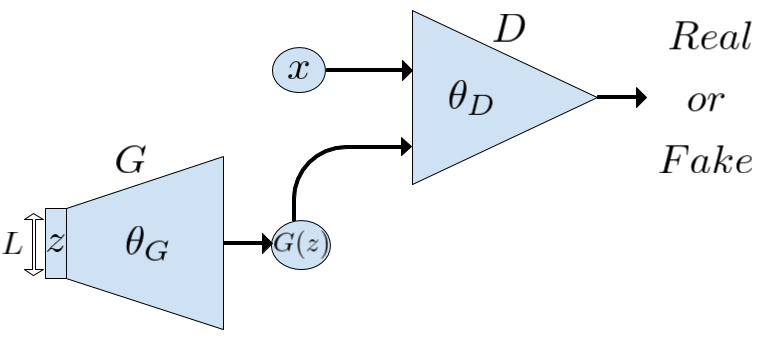
\includegraphics[width=\textwidth]{Figures/GAN/GAN_representation.png}
    \caption{Architecture d'un GAN.}
    \label{fig:fig9}
\end{figure}
Les \textit{Generative Adversarial Networks} (GAN) sont des modèles qui permettent de générer des données approchant une loi de probabilité cible \(P(x)\), où \(x\) est l'ensemble des données que l'on cherche à approcher.

Ces modèles dans la version d'origine présentée par I. Goodfellow~\cite{NIPS2014_5423} se présente sous la forme de deux réseaux distinct : \\
\begin{itemize}
  \item Un générateur \(G\) qui prend en entrée un vecteur aléatoire \(z\) dans un espace latent de dimension \(L\) et produit en sortie des données qui, après un entraînement réussi, doivent approcher la loi de probabilité \(P(x,z)\). Ici l'espace de représentation des données est a l'entrée de \(G\), il s'agit d'un cas spécifique aux GANs. Les poids de \(G\) sont notés \(\theta_G\) (c.f. figure \ref{fig:fig9}) ;
  
  \item Un discriminateur \(D\) qui a pour objectif de calculer la probabilité de \(y\) sachant \(x\), avec \(y\) le label et \(x\) les données. Dans notre cas le label est soit \(0\) pour des données générées soit \(1\) pour des données appartenant a \(x\). Son objectif est donc de déterminer si \(x\) appartiennent au jeu de données ou non. Les poids de \(D\) sont notés \(\theta_D\) (c.f. figure \ref{fig:fig9}) .
\end{itemize}
Ces deux réseaux vont être entraînés en parallèle par rétro-propagation du gradient en minimisant les fonctions de coûts suivantes pour le discriminateur:
$$
lossD = -\log(D(x)) - \log(1-D(G(z))) 
$$
et le générateur
$$
lossG = -\log(D(G(z)))  \\
$$
Ces deux fonctions de coût se rapportent dans notre cas à la fonction de \textit{Binary Cross Entropy} qui mesure la distance (en bits) à l'optimum de chaque composant tel que : 
\[
BCE(a, b) = -[b * \log(a) + (1 - b) * \log(1 - a)]
\]
Avec \(a\) les réponses données par \(D\) pour des images et \(b\) les réponses attendues pour ces images.

\newpage
Pour entraîner les deux réseaux, on suit l'algorithme suivant :
\begin{table}[h!]
  \begin{tabular}{l}
  \hline
  Algorithme 1: Entraînement d'un GAN\tabularnewline
  \hline
  Entrées: Nombre d'itération de l'entraînement  \(I\), la taille des batchs \(B\), le jeu de données \(data\)  \tabularnewline
  Sortie: G un générateur entraîné \tabularnewline
  \hline
  Pour \(I\) étapes faire :\tabularnewline 
  \hspace{1cm}\(z \leftarrow\) ensemble de \(B\) vecteur de taille \(L\) \(\sim \mathcal{N}(0,1)\)\tabularnewline
  \hspace{1cm}\(imagesGenerees \leftarrow\) \(G(z)\)\tabularnewline  
  \hspace{1cm}\(imagesReelles \leftarrow\) échantillon de \(B\) images de \(data\)\tabularnewline
  \hspace{1cm}\(Fake \leftarrow\) vecteur de taille \(B\) initialisé à 0\tabularnewline
  \hspace{1cm}\(Valid \leftarrow\) vecteur de taille \(B\) initialisé à 1\tabularnewline
  \tabularnewline
  \hspace{1cm}\# Entraînement de D\tabularnewline
  \hspace{1cm}\(d_x \leftarrow D(imagesReelles)\)\tabularnewline
  \hspace{1cm}\(d_{g_z} \leftarrow D(imagesGenerees)\)\tabularnewline
  \hspace{1cm}\(lossD \leftarrow BCE(d_x,Valid) + BCE(d_{g_z},Fake)\)\tabularnewline
  \hspace{1cm}Utilisation de \(lossD\) pour mettre à jour \(\theta_D\) par descente de gradient stochastique\tabularnewline
  \tabularnewline
  \hspace{1cm}\# Entraînement de G\tabularnewline
  \hspace{1cm}\(lossG\leftarrow BCE(d_{g_z},Valid)\)\tabularnewline
  \hspace{1cm}Utilisation de \(lossG\) pour mettre à jour \(\theta_G\) par descente de gradient stochastique\tabularnewline
  \tabularnewline
  return G\tabularnewline
  \hline
  \end{tabular}
  \label{tab:tab1}
\end{table}

L'algorithme utilisé pour effectuer les descentes de gradient lors de nos expériences est \href{https://arxiv.org/pdf/1412.6980.pdf}{ADAM}~\cite{kingma2014adam}. Des tests ont été réalisés avec une descente de gradient stochastique standard sans changement qualitatitaif notable dans l'entraînement. ADAM est tout de même plus rapide et il a donc été choisi par défaut.
\subsection{Limites théoriques des GANs}
\label{sec:CompEtLimites}
Une part importante de nos recherches a consisté à essayer de comprendre les barrières théoriques qui entourent les GANs et leurs apprentissages. Les difficultés rencontrées lors de l'apprentissage d'un GAN sont importantes notamment à cause du grand nombre d'hyper-paramètres (voir section \ref{sec:ParamsScans}) ou encore de la difficulté qu'il y a de mesurer la qualité de l'apprentissage durant l'entraînent. 
En effet, pour les GANs standard, aucune mesure ne permet directement de savoir si les images générées sont cohérentes au vu du jeu de données. L'objectif pratique des GANs n'est pas d'obtenir un générateur qui produise exactement les images du jeu de données, mais plutôt de produire des images à la fois diverses et proches des données. Cette notion de distance entre les images générées et celles du jeu de données est difficile à mesurer. C'est pourquoi la plupart du temps il est nécessaire d'observer les images générées pour juger de la qualité de l'entraînement.

Nous nous sommes également penchés sur le problème dit de \textit{mode collapse}, qui fait référence à un apprentissage lors duquel le générateur se met à produire des images peu diversifiées et souvent incohérentes, compte tenu du jeu de données (c.f. figure \ref{fig:fig7}). Ce problème a notamment été  étudié dans la section 3.2 de~\cite{salimans2016improved} et dans la section 2.4 de~\cite{DBLP:journals/corr/MetzPPS16}.

La difficulté qui existe pour atteindre un point de convergence, dû au fait que l'équilibre de Nash entre les deux réseaux n'est pas garanti, fait également partie des problèmes important rencontrés lors de l'entraînement d'un GAN.
Ces questions seront discutées dans les sections  \ref{sec:ParamsScans}, \ref{sec:Mesure}, \ref{sec:Nash_Collapse}.

\newpage
\subsection{Adversarial Auto-Encoder (AAE)}
\label{sec:AAE}

\begin{figure}[h!]
    \centering
    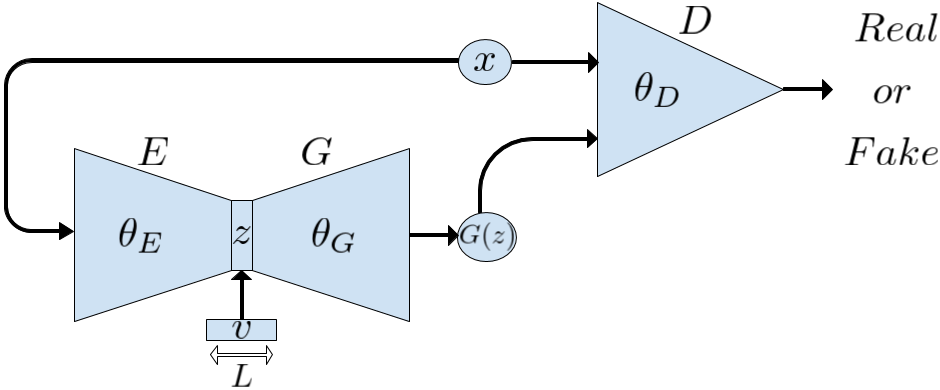
\includegraphics[width=\textwidth]{Figures/GAN/AAE_representation.png}
    \caption{Architecture d'un AAE. Le vecteur \(v\) représente une entrée directe de \(G\) sans passer par \(E\).}
    \label{fig:fig10}
\end{figure}

Pour les expériences sur l'étude des espaces latent que nous allons détailler par la suite (c.f. section \ref{sec:CorrespondancesLS}) nous avons choisi d'utiliser une architecture proche de celle présentée dans l'article de~\cite{GADAE}. Cette architecture nous donne un contrôle sur l'espace latent.
On trouve dans la littérature différentes formes d'auto-encodeurs adversaires, comme par exemple la version de~\cite{makhzani2015adversarial} qui est la plus répandue.

Dans le modèle que nous avons choisi, on trouve dans un premier temps un auto-encodeur (AE), qui est un réseau composer de deux parties symétriques avec en entrée un encodeur \(E\) qui réduit la dimension des données jusqu'à une taille \(L\) et en sortie un décodeur \(G\) qui augmente la taille de ce vecteur de taille \(L\) jusqu'à la taille d'origine des données. 

Nous avons donc dans notre réseau (c.f. figure \ref{fig:fig9}):
\begin{itemize}
  \item un AE comme présenté ci-dessus, avec un encodeur \(E\) (dont les poids seront notés \(\theta_E\)), un décodeur \(G\) qui sert également de générateur (dont les poids seront notés \(\theta_G\)). À la sortie de \(E\) et a l'entrée de \(G\) on trouve un espace latent de taille \(L\);
  \item On associe ce réseau à un discriminateur \(D\) chargé de déterminer si les images qui lui sont présentées viennent du décodeur ou du jeu de données. Les poids de \(D\) sont notés \(\theta_D\) 
\end{itemize}
Les fonctions de coûts utilisées pour entraîner ce réseau sont :
\[
lossD = -\log(D(x)) - \log(1-D(G(z)))
\]
\[
lossG = -\log(D(G(z)))
\]
\[
lossEG = MSE(x, G(E(x))) + MSE(z_{imgs}, z_{zeros}) + MSE(z_{imgs}^2, z_{ones}^2)^{0.5}
\]
Avec MSE définie comme l'erreur quadratique moyenne.
Le \(lossEG\) sera détaillé dans la sous-section suivante \ref{sec:LatentSpace}.

L'intérêt d'un tel dispositif est qu'il permet d'avoir un accès direct à l'espace latent. Ainsi on pourra par la suite mener des expériences sur la façon dont est construit l'espace latent.


On suit un algorithme d'entraînement légèrement diffèrent que pour les GANs standard que voici :\\
\newpage
\begin{table}[t!]
  \begin{tabular}{l}
  \hline
  Algorithme 2: Entraînement d'un AAE\tabularnewline
  \hline
  Entrées: Nombre d'itération de l'entraînement  \(I\), la taille des batchs \(B\), le jeu de données \(data\)  \tabularnewline
  Sortie: G un générateur entraîner \tabularnewline
  \hline
  Pour \(I\) étapes faire :\tabularnewline 
  \hspace{1cm}\(z \leftarrow\) ensemble de \(B\) vecteur de taille \(L\) \(\sim \mathcal{N}(0,1)\)\tabularnewline
  \hspace{1cm}\(imagesGenerees \leftarrow\) \(G(z)\)\tabularnewline  
  \hspace{1cm}\(imagesReelles \leftarrow\) échantillon aléatoire de \(B\) images de \(data\)\tabularnewline
  \hspace{1cm}\(Fake \leftarrow\) vecteur de taille \(B\) initialiser à 0\tabularnewline
  \hspace{1cm}\(Valid \leftarrow\) vecteur de taille \(B\) initialiser à 1\tabularnewline
  \tabularnewline
  
  \hspace{1cm}\# Entraînement de EG\tabularnewline
  \hspace{1cm}\(z_{zeros} \leftarrow\) ensemble de \(B\) vecteur de taille \(L\) initialiser à 0\tabularnewline
  \hspace{1cm}\(z_{ones} \leftarrow\) ensemble de \(B\) vecteur de taille \(L\) initialiser à 1\tabularnewline
  \hspace{1cm}\(z_{imgs} \leftarrow E(imagesReelles)\)\tabularnewline
  \hspace{1cm}\(decoded_{imgs} \leftarrow G(z_{imgs})\)\tabularnewline
  \hspace{1cm}\(lossEG \leftarrow MSE(imagesReelles, decoded_{imgs}) + MSE(z_{imgs}, z_{zeros}) +\)\tabularnewline
  \hspace{2,8cm}\(MSE(z_{imgs}^2, z_{ones}^2)^{0.5}\)\tabularnewline
  \hspace{1cm}Utilisation de \(lossEG\) pour mettre à jour \(\theta_E\) et \(\theta_G\) par descente de gradient stochastique\tabularnewline
  \tabularnewline
  
  \hspace{1cm}\# Entraînement de D\tabularnewline
  \hspace{1cm}\(d_x \leftarrow D(imagesReelles)\)\tabularnewline
  \hspace{1cm}\(d_{g_z} \leftarrow D(imagesGenerees)\)\tabularnewline
  \hspace{1cm}\(lossD \leftarrow BCE(d_x,Valid) + BCE(d_{g_z},Fake)\)\tabularnewline
  \hspace{1cm}Utilisation de \(lossD\) pour mettre à jour \(\theta_D\) par descente de gradient stochastique\tabularnewline
  \tabularnewline
  
  \hspace{1cm}\# Entraînement de G\tabularnewline
  \hspace{1cm}\(lossG\leftarrow BCE(d_{g_z},Valid)\)\tabularnewline
  \hspace{1cm}Utilisation de \(lossG\) pour mettre à jour \(\theta_G\) par descente de gradient stochastique\tabularnewline
  \tabularnewline
  
  return G\tabularnewline
  \hline
  \end{tabular}
  \label{tab:tab2}
\end{table}


\subsection{Contraindre l'espace latent de l'auto-encodeur}
\label{sec:LatentSpace}
%lien avec VAE de Kingma \url{https://arxiv.org/pdf/1312.6114.pdf}
Le \(lossEG\) s'inspire d'un article de Kingma~\cite{kingma2013auto} dans lequel est détaillé une méthode permettant notamment de contraindre une loi de probabilité quelconque à suivre une loi Gaussienne. Grâce à cet outil, on s'assure que l'espace latent \(z\) au centre de l'auto-encodeur suive une loi Gaussienne, et plus particulièrement normale, c'est à dire de moyenne nulle et de variance l'unité. Ceci nous permettra par la suite d'utiliser le générateur (qui est le décodeur de l'AE) en lui donnant des vecteurs suivants une loi normale. Ainsi l'espace latent de l'AE et celui du générateur correspondront.
En créant cette correspondance entre les deux espaces latents on pourra les étudier en détail, ce qui sera le sujet de l'une des expériences que nous présentons dans la section \ref{sec:CorrespondancesLS}.

%%%%%%%%%%%%%%%%%%%%%%%%%%%%%
\section{Méthodes}

\subsection{Exploration des hyper-paramètres}
\label{sec:ParamsScans}
L'ensemble des paramètres d'ajustement des algorithmes d'apprentissage et d'optimisation seront appelés hyper-paramètres. Il ne s'agit donc pas des poids du réseau que l'on optimise durant l'entraînement, mais des paramètres qui définiront la façon dont seront optimisés ces poids.\\
Pour bien comprendre le gigantisme de l'espace des paramètres : on peut vouloir tester le taux d'apprentissage (\textit{learning rate}) du générateur pour des valeurs allant de 0.00005 à 0.005 avec un pas de 0.00005. Ce qui nous ferait une centaine de modèles a entraîner sans même compter tous les autres hyper-paramètres tels que le niveaux de normalisation par batch (\textit{batchNormalization}), le nombre de convolution ou encore leurs tailles.\\
Le nombre important d'hyper-paramètres présent dans les GANs nous a poussé a développer un outil permettant de passer en revue un nombre important de paramètres pour un GAN donné.
Ainsi nous avons pu parcourir de manière efficace ces immenses espaces de paramètres. Nous avons par la suite très largement utilisé cet outil pour régler nos GANs durant toutes les expériences qui seront décrites plus bas.

\subsection{Simpsons Dataset}
\label{sec:SimpsonsDataset}
Pour certaines de nos expériences nous avons utilisé le jeu de données \href{https://www.kaggle.com/kostastokis/simpsons-faces}{Simpsons Faces} \footnote{\label{note2}Simpsons Faces : https://www.kaggle.com/kostastokis/simpsons-faces}. Ce jeu de données contient 9877 images de visage des personnages des Simpsons extrait des épisodes de manière automatique. Ce processus a introduit un certain nombre d'erreurs dans les données (aucun personnage sur l'image, des visages coupés, ect...), pour cette raison j'ai effectué une passe manuelle pour retirer au maximum ces mauvaises images du jeu de données et nous avons finalement utilisé 9629 images pour nos expériences. Vous pouvez voir quelques exemples d'images de ce jeu de données sur la figure \ref{fig:fig1}.\\
Après des tests avec des résolutions plus faibles nous avons choisi d'utiliser ces images en taille 128x128 pixels pour nos expériences. Le procédé fonctionne peu importe la taille des images, mais 128x128 pixels a été un bon compromis entre résolution des images et temps de calcul.

\begin{figure}[!h]
    \centering
    \begin{subfigure}[b]{0.19\textwidth}
        
\includegraphics[width=\textwidth]{Figures/Simpsons_Dataset/13.png}
    \end{subfigure}
    \begin{subfigure}[b]{0.19\textwidth}
        
\includegraphics[width=\textwidth]{Figures/Simpsons_Dataset/15.png}
    \end{subfigure}
    \begin{subfigure}[b]{0.19\textwidth}
        
\includegraphics[width=\textwidth]{Figures/Simpsons_Dataset/25.png}
    \end{subfigure}
    \begin{subfigure}[b]{0.19\textwidth}
        
\includegraphics[width=\textwidth]{Figures/Simpsons_Dataset/8.png}
    \end{subfigure}
    \begin{subfigure}[b]{0.19\textwidth}
        
\includegraphics[width=\textwidth]{Figures/Simpsons_Dataset/18.png}
    \end{subfigure}
    \caption{Exemples d'images du jeu de données Simpsons Faces utilisé pour certaines expériences.}
    \label{fig:fig1}
\end{figure}

\subsection{Simpsons Generator}
\label{sec:SimpsonsGenerator}
La première partie du stage à consisté en une exploration du monde des GANs. Nous nous sommes donc fixé comme objectif la recherche, l'étude et l'entraînement d'un modèle capable de générer des visages de personnages des Simpson.
Après avoir choisi notre jeu de données nous avons exploré l'immense monde des GANs et nous avons rapidement dû faire des choix étant donné la quantité astronomique d'articles présentant des variantes de GAN (c.f. \href{https://github.com/hindupuravinash/the-gan-zoo}{The Gan Zoo} \ref{note1}).
Nous avons donc focalisé notre attention sur les systèmes les plus éprouvés afin de comprendre au mieux la théorie derrière ces modèles.

Nous avons particulièrement utilisé les DCGAN~\cite{radford2015unsupervised} qui sont notamment composés de couches de convolution très adaptées au traitement des images. Puis dans un second temps nous nous sommes penchés sur les \textit{Adversarial Auto-Encoders} (AAE) qui nous on servi par la suite pour l'expérience présentée en section \ref{sec:CorrespondancesLS}.

\subsection{Fractal Dream Dataset}
\label{sec:FDD}
Pour l'une des expériences que nous souhaitions mener (c.f. section \ref{sec:CorrespondancesLS}), nous avions besoin d'un jeu de données paramétrique. 
En effet il nous fallait un jeu de données dont chaque image puisse être associées à un point dans l'espace de manière cohérente. 
Pour ce faire nous avons décidé de construire un nouveau jeu de données à partir d'un outil mathématique : les attracteurs étranges~\cite{Pickover}. Ces objets permettent notamment de générer des figures variées à partir d'un nombre donné de paramètres.
Les Fractal Dream~\cite{Pickover} sont un type particulier d'attracteur étrange que nous avons choisi pour notre jeu de données. À partir de six paramètres, la formule disponibles en annexes \ref{appendix:annexe1} permet de calculer de manière itérative (pour un nombre d'itération donner) un ensemble de points qui constitue la trajectoire de l'attracteur. Une fois ces points placés dans un quadrillage de taille finie (128x128 dans notre cas) on obtient une image comme celles visibles dans la figure \ref{fig:fig2}. Dans les images les nuances de couleurs des pixels correspondent aux nombres de fois ou l'attracteur est passé dans la case. 
Le jeu de données est constitué de trois classes d'images correspondant aux trois palettes de couleurs choisis (bleu, orange et vert), pour nos expériences nous n'avons utilisé qu'une seule de ces trois palettes pour faciliter l'entraînement.\\
Le jeu de données construit pour l'occasion ainsi que les codes utilisés on était mis à disposition sur le site Kaggle : \href{https://www.kaggle.com/lgoareguer/fractal-dream-dataset}{Fractal Dream Dataset} \footnote{\label{note3}Fractal Dream Dataset : https://www.kaggle.com/lgoareguer/fractal-dream-dataset}.

\begin{figure}[h!]
    \centering
    \begin{subfigure}[b]{0.20\textwidth}
        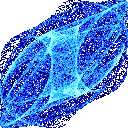
\includegraphics[width=\textwidth]{Figures/FDD/-0,00545687187361743_-0,5312304575586382_1,8197494653032407_2,422111729355857_1,4944898296889655_2,487490210145214.png}
    \end{subfigure}
    \begin{subfigure}[b]{0.20\textwidth}
        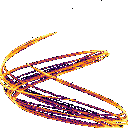
\includegraphics[width=\textwidth]{Figures/FDD/-0,319459804135373_-0,0981842500805612_0,42291442353441633_1,7253282321258185_1,4272325555244099_1,3701336149016234.png}
    \end{subfigure}
    \begin{subfigure}[b]{0.20\textwidth}
        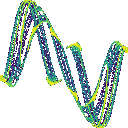
\includegraphics[width=\textwidth]{Figures/FDD/-0,9333646250089_-0,3698044331245828_-1,9514116449042127_-0,376713271698188_-1,1759178511809651_-1,7157801385982319.png}
    \end{subfigure}
    \caption{Exemples d'images du jeu de données Fractal Dream Dataset utilisé pour certaines expériences. Vous pourrez trouver la liste des paramètres utilisés pour générer ces trois figures en annexes \ref{appendix:annexe1}.}
    \label{fig:fig2}
\end{figure}

\subsection{Correspondances des espaces latents}
\label{sec:CorrespondancesLS}
Nous nous sommes posé de nombreuses question concernant la façon dont est construit l'espace latent des GANs. 
Nous avons notamment voulu savoir si étant donné une base de données \(data\) composée d'images \(x\), chacune associée à un unique vecteur \(v\), de dimension \(L\), répartie de manière cohérente dans l'espace. Un générateur \(G\) entraîné avec un AAE, pourrait-il générer une image \(x'\) proche de celle d'une image \(x\) pour un même vecteur \(v\) ? Autrement dit : le générateur serait-il capable de reconstruire, par un entraînement adversaire, la fonction qui relie les images de \(data\) au vecteur \(v\) qui leur est associé. Pour mettre en place cette expérience nous avons entraîné un AAE avec le jeu de données FDD présenté dans la section \ref{sec:FDD}. Ensuite, nous avons pu comparer les images de FDD aux images générées par \(G\) pour un même vecteur \(v\). La figure \ref{fig:fig11} décris cette expérience.

\begin{figure}[!h]
    \centering
    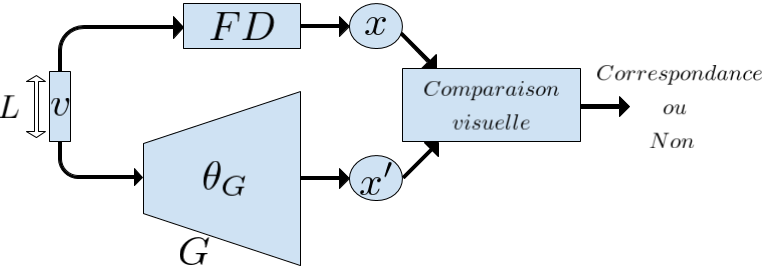
\includegraphics[width=\textwidth]{Figures/CorrespondancesLS/CorrespondancesLS.png}
    \caption{Description de l'expérience de comparaison des espaces latents. Ici FD correspond à l'opération permettant de calculer une image de type Fractal Dream.}
    \label{fig:fig11}
\end{figure}


%%%%%%%%%%%%%%%%%%%%%%%%%%%%%
\section{Résultats}
\subsection{Simpsons Cohérent}
\label{sec:SimpsonsCoherent}

Le balayage des hyper-paramètres ainsi que l'affinage des modèles au grès de nos recherches ont permis d'obtenir de très bons résultats. Vous pouvez voir sur la figure \ref{fig:fig3} les résultats obtenus avec un DCGAN et sur la figure \ref{fig:fig4} les résultats obtenus avec un AAE. 
Il faut noter que les deux modèles étant diffèrent ils disposent d'hyper-paramètres adapter, mais nous avons cherché a leurs données des capacités similaires (même nombre de couches pour \(G\) et \(D\), même nombre de filtres par convolution,etc...). L'objectif était de pouvoir comparer les deux architecture sur le plan de la génération d'images et sur ce point les AAE montrent des capacités moindre que les DCGAN.
On constate ici et dans chacune de nos expériences que les images obtenues avec l'AAE présente un aspect flou. Ceci vient certainement du fait que la fonction de coût de l'AE rentre en opposition (ou du moins n'est pas en totale adéquation) avec la fonction de coût du générateur qui est affecter par les deux.

\begin{figure}[!h]
 \centering
    \begin{subfigure}[b]{\textwidth}
        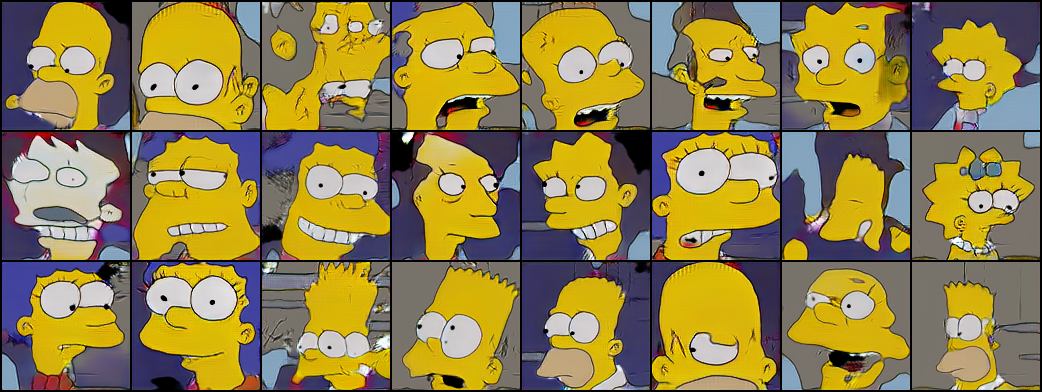
\includegraphics[width=\textwidth]{Figures/resultats_simpsons/DCGAN_270.png}
        \caption{Images générées avec le générateur d'un DCGAN.}
        \label{fig:fig3}
    \end{subfigure}
    \begin{subfigure}[b]{\textwidth}
        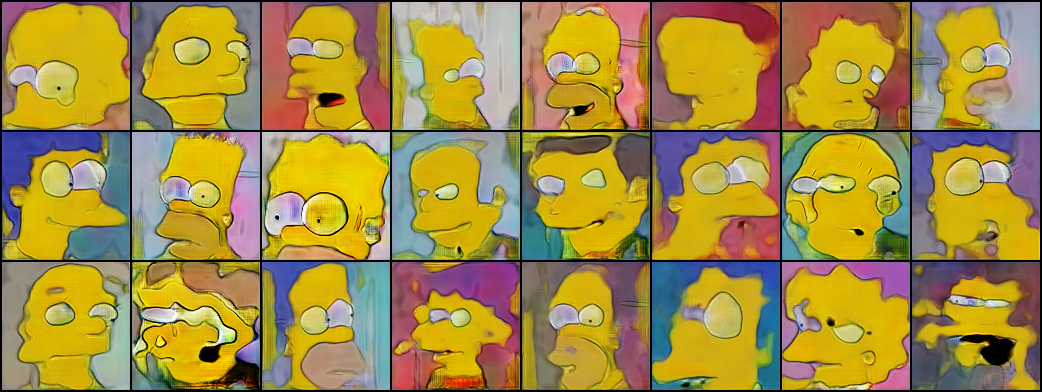
\includegraphics[width=\textwidth]{Figures/resultats_simpsons/AAE_300.png}
        \caption{Images générées avec le générateur d'un AAE.}
        \label{fig:fig4}
    \end{subfigure}
    \caption{Images générer par deux générateur entraîner différemment.}
\end{figure}

\subsection{Mesure de la qualité des résultats}
\label{sec:Mesure}

Malgré l'importante quantité de travaux sur le sujet, les GANs laissent encore planer de nombreuses questions. 
Durant nos expériences nous nous sommes confronté à de nombreuse barrières théoriques qui ne sont pas encore tombées.\\
L'une des principales faiblesses des GANs est l'absence de mesure de la qualité des résultats. En effet même si dans la section 4.2 de l'article~\cite{NIPS2014_5423}, \(G\) est sensé converger vers un point où les données qu'il génère suive la loi de probabilités du jeu de données, dans la pratique aucun point de convergence n'est atteint entre \(G\) et \(D\). Ceci est dû notamment au fait que \(G\) n'apprend que par le biais de \(D\), il n'a donc pas pour objectif de se rapprocher des données du jeu de données, mais de générer des données qui trompent \(D\). On ne peut donc pas ce fier au fonction de coût de \(G\) pour évaluer son niveau d'apprentissage. 
Certain article se sont focalisés sur la recherche d'une métrique adaptée aux GANs comme dans~\cite{salimans2016improved} qui utilise ce qu'ils appellent l'Inception score pour évaluer les images ou encore~\cite{berthelot2017began} qui introduit une nouvelle architecture de GAN ainsi qu'une métrique associée.\\

\subsection{Équilibre de Nash et \textit{mode collapse}}
\label{sec:Nash_Collapse}
A ce problème de mesure s'ajoute un problème d'équilibre. 
En effet comme dit précédemment on peut voir l'apprentissage de notre réseaux comme un jeu a somme nul dans lequel ce que \(G\) gagne \(D\) le perd et inversement.\\
L'objectif de ce jeu est donc d'atteindre le point d'équilibre tel que \(G\) produit un résultat suivant la loi de probabilité \(P(x\)). Dans ce cas \(D\) devient incapable de différencier les images générée par \(G\) des images du jeu de données. Ici l'entraînement est terminé et \(G\) produit les images attendues. L'équilibre de Nash est atteint.\\
Malheureusement ce que nos expériences nous ont apprises c'est que cet état d'équilibre, s'il existe, n'est jamais atteint (dans le cadre de nos expériences en tout cas).\\
Comme vous pouvez le voir sur la figure \ref{fig:fig5} la moyenne des réponses du discriminateur pour les images réelles et pour les images générées tend vers un point où \(D\) ne fait presque plus aucune erreur. Étant donné que \(G\) apprend via les réponses de \(D\) on constate que la fonction de coût de \(G\) devient de plus en plus proche de l'infini ce qui à tendance à créer une forte instabilité dans l'apprentissage. Cette instabilité peut être observée sur la figure \ref{fig:fig6} où l'on constate que plus l'apprentissage ce prolonge plus la fonction de coût de \(G\) devient inconstant.
En effet \(G\), dû fait de sa fonction de coût \ref{sec:GAN}, a besoin que \(D\) réussisse à discriminer les images générées pour pouvoir se corriger et s'adapter. Mais plus \(D\) réussis à classer correctement les images plus \(G\) obtient une fonction de coût importante ce qui le pousse au déséquilibre. C'est ce que l'on appelle dans le monde des GANs un \textit{mode collapse}. Vous pouvez voir sur la figure \ref{fig:fig7} un exemple d'images générer lors du \textit{mode collapse} d'un générateur. On constate que la diversité des images devient pauvre et totalement incohérente. Ce phénomène s'explique, par le fait que \(D\), fini par réussir tellement bien à classer les images, qu'il pousse \(G\) à se focaliser sur les quelques images qui réussissent encore a trompées \(D\). Ainsi \(G\) ce met a générer une seule (ou très peut) d'images ce qui veut dire que l'espace latent de \(G\) devient très uniforme. De nombreux articles on étudier le \textit{mode collapse} comme par exemple~\cite{NIPS2014_5423}.\\
Fort heureusement cet absences d'équilibre n'empêche pas l'entraînement du générateur. Il est vraie que \(D\) fini toujours (dans nos expériences) par prendre l'avantage et ne fait presque plus aucune erreur, mais \(G\) réussis encore, rarement, a flouée \(D\). Le fait que \(G\) réussisse a gagner face a un générateur bien meilleurs que lui, lui permet de continuer son apprentissage. Les victoires de \(G\), même si elle sont rare, permettent a \(D\) de s'améliorer puis les victoires de \(D\) permettent a leur tours à \(G\) de s'améliorer. \\
\newpage
\begin{figure}[!h]
 \centering
    \begin{subfigure}[b]{\textwidth}
        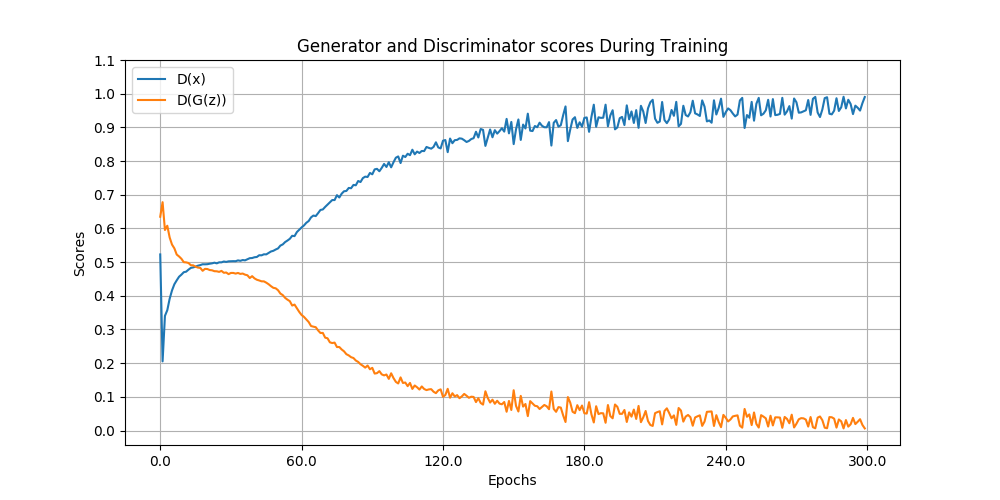
\includegraphics[width=0.85\textwidth]{Figures/LossG_et_Convergeance/scores300-64.png}
        \caption{Moyenne des réponses de \(D\) pour les images réels en bleu et les images générées en orange, au cours de l'entraînement.}
        \label{fig:fig5}
    \end{subfigure}
    \begin{subfigure}[b]{\textwidth}
        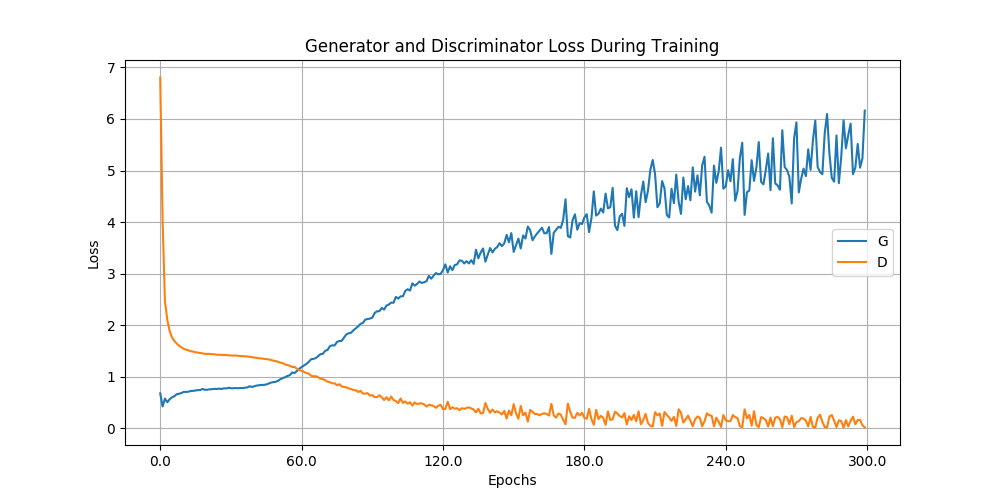
\includegraphics[width=0.85\textwidth]{Figures/LossG_et_Convergeance/losses300-64.png}
        \caption{Valeurs des fonctions de coûts de \(G\) (en bleu) et \(D\) (en orange), au cours de l'entraînement.}
        \label{fig:fig6}
    \end{subfigure}
    \caption{Courbes des coûts et des scores au cours de l'entraînement.}
\end{figure}

\begin{figure}[h!]
    \centering
    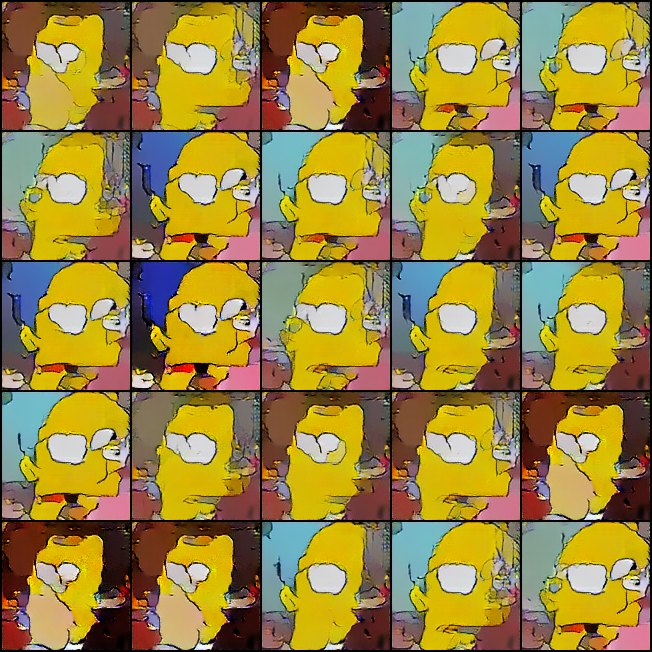
\includegraphics[width=0.40\textwidth]{Figures/LossG_et_Convergeance/collapse_980.png}
    \caption{Exemples d'images générer lors du \textit{mode collapse} d'un générateur. On constate une faible diversité ainsi qu'une incohérence des images par rapport au jeu de données.}
    \label{fig:fig7}
\end{figure}

\subsection{Comparaison des espaces latents connu et générer}
\label{sec:ComparaisonLS}
Vous pouvez voir sur la gauche de la figure \ref{fig:fig8} des images extraite du jeu de données FDD. Après avoir entraîné et paramétré différents modèles à générer des images cohérentes par rapport à celles du jeu de données nous avons pu générer les images visibles à droite et au centre de la figure \ref{fig:fig8}. 
En comparant ces images avec celle de gauche on ne constate aucune correspondance entre celles générer par G et celles construite en utilisant les formules Fractal Dream \ref{sec:FDD}. 
Ce résultat tend a montrer que l'espace latent de G n'a pas développé de correspondance avec l'espace des paramètres de FDD durant sont entraînement.

\begin{figure}[!h]
    \centering
    \begin{subfigure}[b]{0.32\textwidth}
        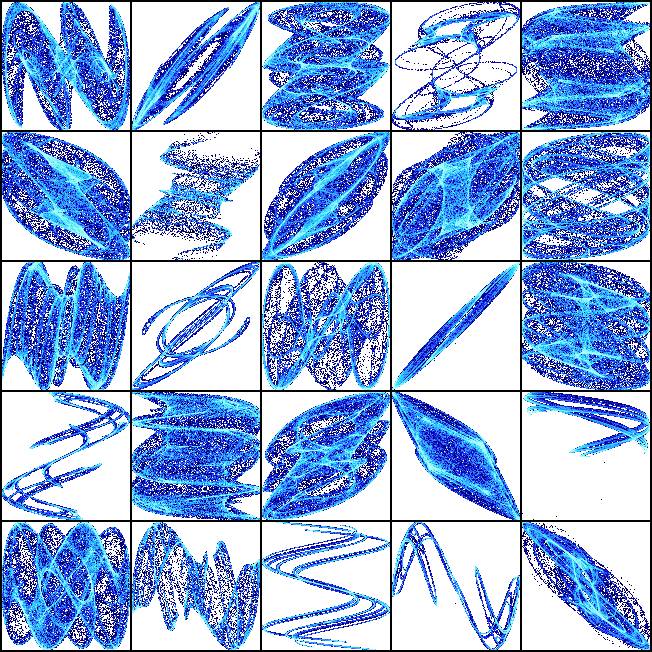
\includegraphics[width=\textwidth]{Figures/ComparaisonLS/dataset_sample.png}
        \caption{Des éléments extraits du jeu de données Fractal Dream Dataset.}
    \end{subfigure}
    \begin{subfigure}[b]{0.32\textwidth}
        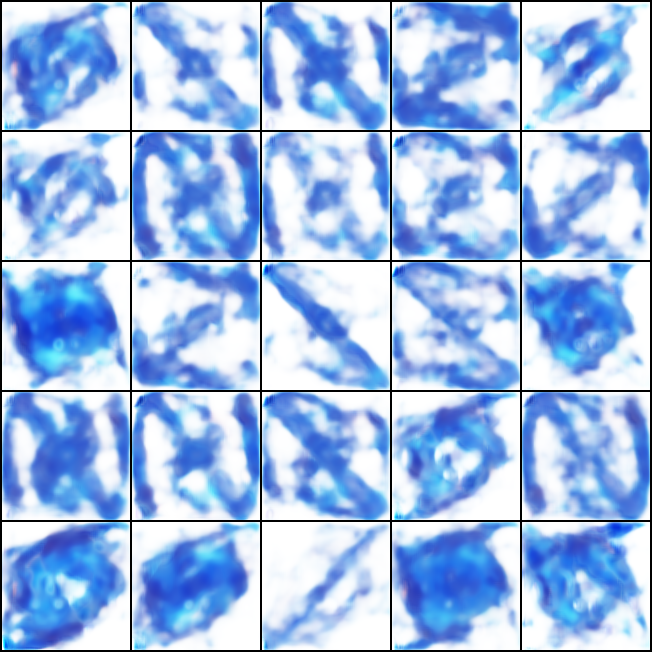
\includegraphics[width=\textwidth]{Figures/ComparaisonLS/scan7_eps0,1_lrelu0,01_0.png}
        \caption{Des images générées par un générateur entraîné par un AAE.}
    \end{subfigure}
    \begin{subfigure}[b]{0.32\textwidth}
        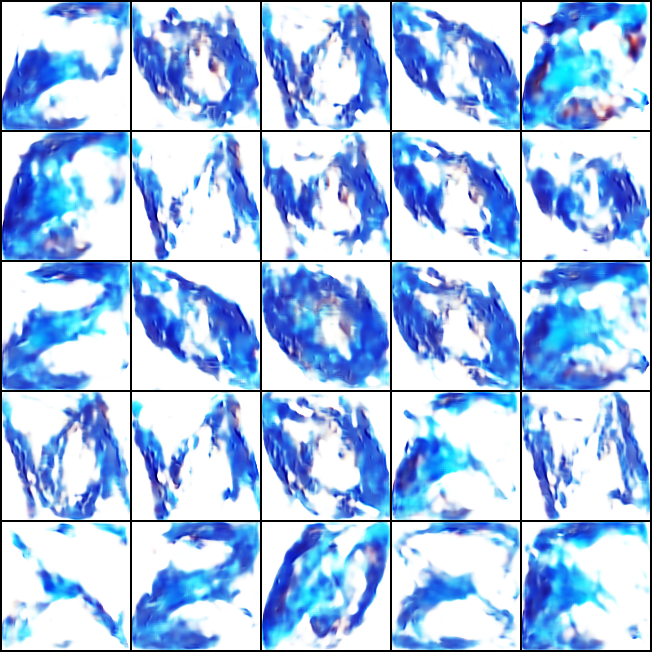
\includegraphics[width=\textwidth]{Figures/ComparaisonLS/scan8_eps0,1_lrelu1e06_0.png}
        \caption{Des images générées par un autre générateur entraîné par un AAE.}
    \end{subfigure}
    \caption{Les images générées l'on était en utilisant un vecteur latent correspondant aux paramètres utiliser pour calculer les images extraite du jeu de données visible à droite.}
    \label{fig:fig8}
\end{figure}
%\subsection{Interpolation dans l'espace latent}

%%%%%%%%%%%%%%%%%%%%%%%%%%%%%
\section{Conclusions et perspectives}
\label{sec:Conclusion}

\subsection{Apprentissage des GANs}
L'apprentissage des GANs est une tâche ardue et nous avons eu besoin de beaucoup de test avant d'arriver à un résultat un tant soit peu convaincant. Le grand nombre d'hyper-paramètres ainsi que les vides théoriques présentés section \ref{sec:CompEtLimites} posent de nombreuses difficultés. Néanmoins les résultats obtenus, avec les Simpsons notamment, sont tout à fait convaincant.

\subsection{Découverte et prise en mains de nombreux outils}
Durant le stage j'ai été amené à me former a de nombreuse technologies et outils. On peut citer parmi les plus importants Pytorch~\cite{paszke2017automatic} ou encore Tensorboard~\cite{tensorflow2015-whitepaper}, à ceci s'ajoute également un usage quotidien de Linux et de Python qui m'ont permis de découvrir de nombreux logiciels et bibliothèques. Ensemble ces outils s'agrègent à ceux utilisés lors de mon Master et me permettront, je l'espère, de commencer ma vie professionnelle sur de bonnes bases.

\subsection{Premier pas dans le monde professionnels}
Les laboratoires de recherche sont un monde particulier que j'avais déjà pu approcher lors de mes études, ce stage m'a permis de les découvrir en détails. J'ai pu apprendre tout ce qui fait le monde professionnel : horaires fixes, journée complètes, réunions de travail ect... 
Ces nouvelles expériences forme le début de mon parcours professionnel.

\newpage
%{\bf Appendices}: Appendices, if any, directly follow the text and the references (but see above).  Letter them in sequence and provide an informative title: {\bf Appendix A. Title of Appendix}.
%\section*{Acknowledgements}

%The acknowledgements should go immediately before the references.  Do
%not number the acknowledgements section. Do not include this section
%when submitting your paper for review.

\section*{Remerciements}
Je tiens à remercier Laurent Perrinet pour m'avoir encadrés et guidés durant ce Stage.
Ainsi que Victor Boutin pour ces précieux conseils lors de la rédaction de ce rapport.

\bibliography{biblio}
\bibliographystyle{acl}
%%%%%%%%%%%%%%%%%%%%%%%%%%%%
\newpage

\section{Annexes}
\begin{appendix}
\section{-  Formule des Fractal Dream}
\label{appendix:annexe1}
La formule ci-dessous permet de calculer le point suivant d'un attracteur de type Fractal Dream à partir des coordonnées du point actuel et de quatre paramètres données. 
En utilisant cette formule successivement un grand nombre de fois on peut calculer l'image correspondant à l'attracteur pour des paramètres et un point de départ choisi.

    \begin{table}[hb]
      \begin{tabular}{l}
      \hline
      Algorithme 3: Calcul du point suivant d'un Fractal Dream\tabularnewline
      \hline
      Entrées: \((x, y)\) coordonnées du point courant, \((a, b, c, d)\) paramètres de l'attracteur \tabularnewline
      Sortie: \((x', y')\) les coordonnées du point suivant\tabularnewline
      \hline
      \(x' \leftarrow sin(y*b)+c*sin(x*b)\)\tabularnewline
      \(y' \leftarrow sin(x*a)+d*sin(y*a)\)\tabularnewline
      \tabularnewline
      return \((x', y')\)\tabularnewline
      \hline
      \end{tabular}
      \label{tab:tab3}
    \end{table}
    
Pour l'exemple les paramètres utiliser pour générer les trois images de la figure \ref{fig:fig2} sont respectivement :\\
 1 : \(x = -0,00545687187361743 ~y = -0,5312304575586382 ~a = 1,8197494653032407 ~b = 2,422111729355857 ~c = 1,4944898296889655 ~d = 2,487490210145214\)\\
 2 : \( ~x = -0,319459804135373 ~y = -0,0981842500805612 ~a = 0,42291442353441633 ~b = 1,7253282321258185 ~c = 1,4272325555244099 ~d = 1,3701336149016234\)\\
 3 :  \(~x = -0,9333646250089 ~y = -0,3698044331245828 ~a = -1,9514116449042127 ~b = -0,376713271698188 ~c = -1,1759178511809651 ~d = -1,7157801385982319\)

\section{-  Détail des hyper-paramètres des réseaux}
\label{appendix:annexe2}
Les réseaux on était entraîner avec les hyper-paramètres suivants pour les expériences sur les Simpson :
\begin{itemize}
  \item DCGAN :
  \begin{itemize}
    \item LeakyReLU : factor=1e-6
    \item BatchNorm2d : epsilon=0.5
    \item BatchSize : 16
    \item Learning rate D : 5e-5 
    \item Learning rate G : 2.5e-4
  \end{itemize}
  
  \item AAE :
  \begin{itemize}
    \item LeakyReLU : factor=0.1
    \item BatchNorm2d : epsilon=0.01
    \item BatchSize : 16
    \item Learning rate D : 4e-5 
    \item Learning rate G : 4e-4
    \item Learning rate E : 4e-4
  \end{itemize}
\end{itemize}

\section{-  Détail de l'architecture des réseaux}
\label{appendix:annexe3}
Vous trouverez ci-dessous un détail couches par couches de l'architecture des réseaux DCGAN et AAE ayant servie pour nos expériences.
Les noms des fonction utiliser sont ceux de la librairie Pytorch en version 1.1.0.

\begin{table}[h]
  \begin{tabular}{l}
  \hline
  Input : (16x32) (BatchSize x Latent space size) \tabularnewline
  \hline
  \hline
  Linear : in:32 out:64x512\tabularnewline
  LeakyReLU\tabularnewline
  \hline
  UpsamplingNearest2d : scale factor 2\tabularnewline
  Conv2d : filtres (512)\(\rightarrow\)(256) kernel size=(9, 9), stride=(2, 2), padding=(4, 4) \tabularnewline
  BatchNorm2d\tabularnewline
  LeakyReLU \tabularnewline
  \hline
  UpsamplingNearest2d : scale factor 2\tabularnewline
  Conv2d : filtres (256)\(\rightarrow\)(128) kernel size=(9, 9), stride=(2, 2), padding=(4, 4) \tabularnewline
  BatchNorm2d\tabularnewline
  LeakyReLU \tabularnewline
  \hline
  UpsamplingNearest2d : scale factor 2\tabularnewline
  Conv2d : filtres (128)\(\rightarrow\)(64) kernel size=(9, 9), stride=(2, 2), padding=(4, 4) \tabularnewline
  BatchNorm2d\tabularnewline
  LeakyReLU \tabularnewline
  \hline
  Conv2d : filtres (64)\(\rightarrow\)(3) kernel size=(9, 9), stride=(2, 2), padding=(4, 4) \tabularnewline
  Tanh\tabularnewline
  \hline
  \hline
  Output : (16x3x128x128) (BatchSize x channels x Image size x Image size)\tabularnewline
  \hline
  \end{tabular}
  \label{tab:tab4}
  \caption{Détail de l'architecture du générateur du DCGAN et de L'AAE.}
\end{table}

\begin{table}[h]
  \begin{tabular}{l}
  \hline
  Input : (16x3x128x128) (BatchSize x channels x Image size x Image size) \tabularnewline
  \hline
  \hline
  Conv2d : filtres (3)\(\rightarrow\)(64) kernel size=(9, 9), stride=(2, 2), padding=(4, 4) \tabularnewline
  LeakyReLU \tabularnewline
  \hline
  Conv2d : filtres (64)\(\rightarrow\)(128) kernel size=(9, 9), stride=(2, 2), padding=(4, 4) \tabularnewline
  LeakyReLU \tabularnewline
  BatchNorm2d\tabularnewline
  \hline
  Conv2d : filtres (128)\(\rightarrow\)(256) kernel size=(9, 9), stride=(2, 2), padding=(4, 4) \tabularnewline
  LeakyReLU \tabularnewline
  BatchNorm2d\tabularnewline
  \hline
  Conv2d : filtres (256)\(\rightarrow\)(512) kernel size=(9, 9), stride=(2, 2), padding=(4, 4) \tabularnewline
  LeakyReLU \tabularnewline
  BatchNorm2d\tabularnewline
  \hline
  Linear : in:64x512 out:1\tabularnewline
  \hline
  \hline
  Output : (16x1) (BatchSize x \(D\) answer size)\tabularnewline
  \hline
  \end{tabular}
  \label{tab:tab5}
  \caption{Détail de l'architecture du discriminateur du DCGAN et de L'AAE.}
\end{table}

\begin{table}[h]
  \begin{tabular}{l}
  \hline
  Input : (16x3x128x128) (BatchSize x channels x Image size x Image size) \tabularnewline
  \hline
  \hline
  Conv2d : filtres (3)\(\rightarrow\)(64) kernel size=(9, 9), stride=(2, 2), padding=(4, 4) \tabularnewline
  LeakyReLU\tabularnewline
  \hline
  Conv2d : filtres (64)\(\rightarrow\)(128) kernel size=(9, 9), stride=(2, 2), padding=(4, 4) \tabularnewline
  LeakyReLU\tabularnewline
  BatchNorm2d\tabularnewline
  \hline
  Conv2d : filtres (128)\(\rightarrow\)(256) kernel size=(9, 9), stride=(2, 2), padding=(4, 4) \tabularnewline
  LeakyReLU\tabularnewline
  BatchNorm2d\tabularnewline
  \hline
  Conv2d : filtres (256)\(\rightarrow\)(512) kernel size=(9, 9), stride=(2, 2), padding=(4, 4) \tabularnewline
  LeakyReLU\tabularnewline
  BatchNorm2d\tabularnewline
  \hline
  Linear : in:64x512 out:32\tabularnewline
  \hline
  \hline
  Output : (16x32) (BatchSize x Latent space size) \tabularnewline
  \hline
  \end{tabular}
  \label{tab:tab6}
  \caption{Détail de l'architecture de l'encoder de L'AAE.}
\end{table}


\end{appendix}

%%%%%%%%%%%%%%%%%%%%%%%%%%%%


\end{document}
